% Size class file guide: how the size-class master workbook works, with pictures of the real sheets.
% Five 11 x 17 landscape sheets (ledger, 17 x 11 in) drawn in TikZ, in the house style of open-orders-team-review.tex.
%   Sheets 1 to 4 (about 80%): the file at a glance, the Size Class tab, the Set-up tab, how the macro reads the file
%   and what its messages mean.
%   Sheet 5 (about 20%, the most important, drawn with a peach frame): add a new size class to CTL, SSL or MX.
% The pictures are the real workbook output/open-orders-intake-inventory/size-class-master.xlsx, written by
% make_size_class_guide_shots.py into size-class-guide/ (the worked example: CTL 4000&Over, SSL XL Frame, MX >10-15,
% model E145, shaded peach in the pictures only). Facts from the .bas (LoadSizeClassFile, LoadClasses,
% CheckOpenOrdersReportSetup) and make_size_class_master.py.
% Callouts on a picture use a scope whose x and y run 0 to 1 across and down the picture.
% Each sheet is laid out on a 12 x 7.5 in grid and scaled by 4/3 to fill the 16 x 10 in drawing area.
% Build: ./build.sh source/open-orders-intake-inventory/size-class-file-guide.tex
\documentclass[10pt]{article}
\usepackage[paperwidth=17in, paperheight=11in, margin=0.5in]{geometry}
\usepackage[T1]{fontenc}
\usepackage{lmodern}
\usepackage{microtype}
\usepackage{enumitem}
\usepackage[table]{xcolor}
\usepackage{graphicx}
\usepackage{tikz}
\usetikzlibrary{positioning, arrows.meta, calc, fit}
\usepackage[hidelinks, pdftitle={Size Class File Guide}, pdfauthor={Gust F.}]{hyperref}
\graphicspath{{size-class-guide/}}
\pagestyle{empty}
\setlength{\parindent}{0pt}
\hyphenpenalty=10000
\exhyphenpenalty=10000
\setlist[itemize]{label=\textbullet, leftmargin=0.85em, labelsep=0.35em, itemsep=1.5pt, parsep=0pt,
                  topsep=0pt, partopsep=0pt}
\definecolor{headgreen}{HTML}{548235}
\definecolor{bandgreen}{HTML}{E2EFDA}
\definecolor{flagpeach}{HTML}{FCE4D6}
\definecolor{inputyellow}{HTML}{FFFFCC}
\definecolor{alertorange}{HTML}{C55A11}
\tikzset{
  every node/.style={font=\sffamily\small, inner sep=5pt},
  box/.style={draw, line width=0.5pt, fill=white, align=left},
  station/.style={draw, line width=0.5pt, fill=headgreen, text=white, font=\sffamily\bfseries\normalsize,
                  align=left, inner ysep=4pt, text height=1.6ex, text depth=0.45ex},
  flow/.style={-{Stealth[length=9pt, width=6.5pt]}, line width=1.2pt, line join=miter},
  point/.style={-{Stealth[length=6pt, width=4.5pt]}, line width=0.9pt, alertorange},
  % a numbered marker on a picture, matched by the same number in the text beside it
  marker/.style={circle, fill=headgreen, text=white, draw=white, line width=1pt, font=\sffamily\bfseries\small,
               inner sep=0pt, minimum size=0.25in},
  hot/.style={marker, fill=alertorange},
  shot/.style={draw, line width=0.5pt, inner sep=0pt, anchor=north west},
}
\newcommand{\by}[1]{{\footnotesize\itshape #1}\\[3pt]}
\newcommand{\peach}[1]{{\setlength{\fboxsep}{1pt}\colorbox{flagpeach}{\textbf{#1}}}}
\newcommand{\yellow}[1]{{\setlength{\fboxsep}{1pt}\colorbox{inputyellow}{#1}}}
\newcommand{\btn}[1]{{\setlength{\fboxsep}{1.5pt}\fbox{\footnotesize\bfseries #1}}}
\newcommand{\num}[1]{\tikz[baseline=(n.base)]\node(n)[marker, minimum size=0.2in, font=\sffamily\bfseries\footnotesize]{#1};}
\newcommand{\hotnum}[1]{\tikz[baseline=(n.base)]\node(n)[hot, minimum size=0.2in, font=\sffamily\bfseries\footnotesize]{#1};}
\newcommand{\cls}[1]{{\ttfamily #1}}
% title block, one row in the bottom right corner: #1 title, #2 sheet
\newcommand{\titleblock}[2]{%
  \draw[line width=0.5pt] (5.7,0) -- (5.7,0.42) -- (12,0.42);
  \foreach \x in {7.3, 8.95, 9.5, 9.95, 10.75, 11.45} \draw[line width=0.5pt] (\x,0) -- (\x,0.42);
  \foreach \x/\label/\value in {5.7/Title/#1, 7.3/Project/Open Orders by MSA, 8.95/Macro/v2.8, 9.5/Rev./1,
                                9.95/Date/2026-10-16, 10.75/Drawn/Gust F., 11.45/Sheet/#2} {
    \node[anchor=north west, inner sep=0pt, font=\sffamily\fontsize{7}{8}\selectfont] at (\x+0.07,0.36) {\label};
    \node[anchor=south west, inner sep=0pt, font=\sffamily\bfseries\footnotesize] at (\x+0.07,0.07) {\value};
  }}
% sheet heading: #1 title, #2 subtitle
\newcommand{\heading}[2]{%
  \node[anchor=north west, inner sep=0pt, font=\sffamily\bfseries\fontsize{14}{16}\selectfont] at (0.25,7.25) {#1};
  \node[anchor=north west, inner sep=0pt, font=\sffamily\footnotesize] at (0.25,6.88) {#2};}

\begin{document}
% ============================================================================ sheet 1: at a glance
\noindent
\scalebox{1.333333}{%
\begin{tikzpicture}[x=1in, y=1in]
\useasboundingbox (0,0) rectangle (12,7.5);
\draw[line width=0.8pt] (0,0) rectangle (12,7.5);
\heading{The Size Class File at a Glance}
  {\texttt{size-class-master.xlsx}: the master list that gives every model in the Open Orders report its size class.
   Two tabs; the macro reads both.}

% ---------------------------------------------------------------- the four steps, left to right
\node[station, anchor=north west, text width=2.55in] (h1) at (0.25,6.4) {1\quad Set-up tab};
\node[box, anchor=north, text width=2.55in] (b1) at (h1.south) {\by{Which size classes exist}
  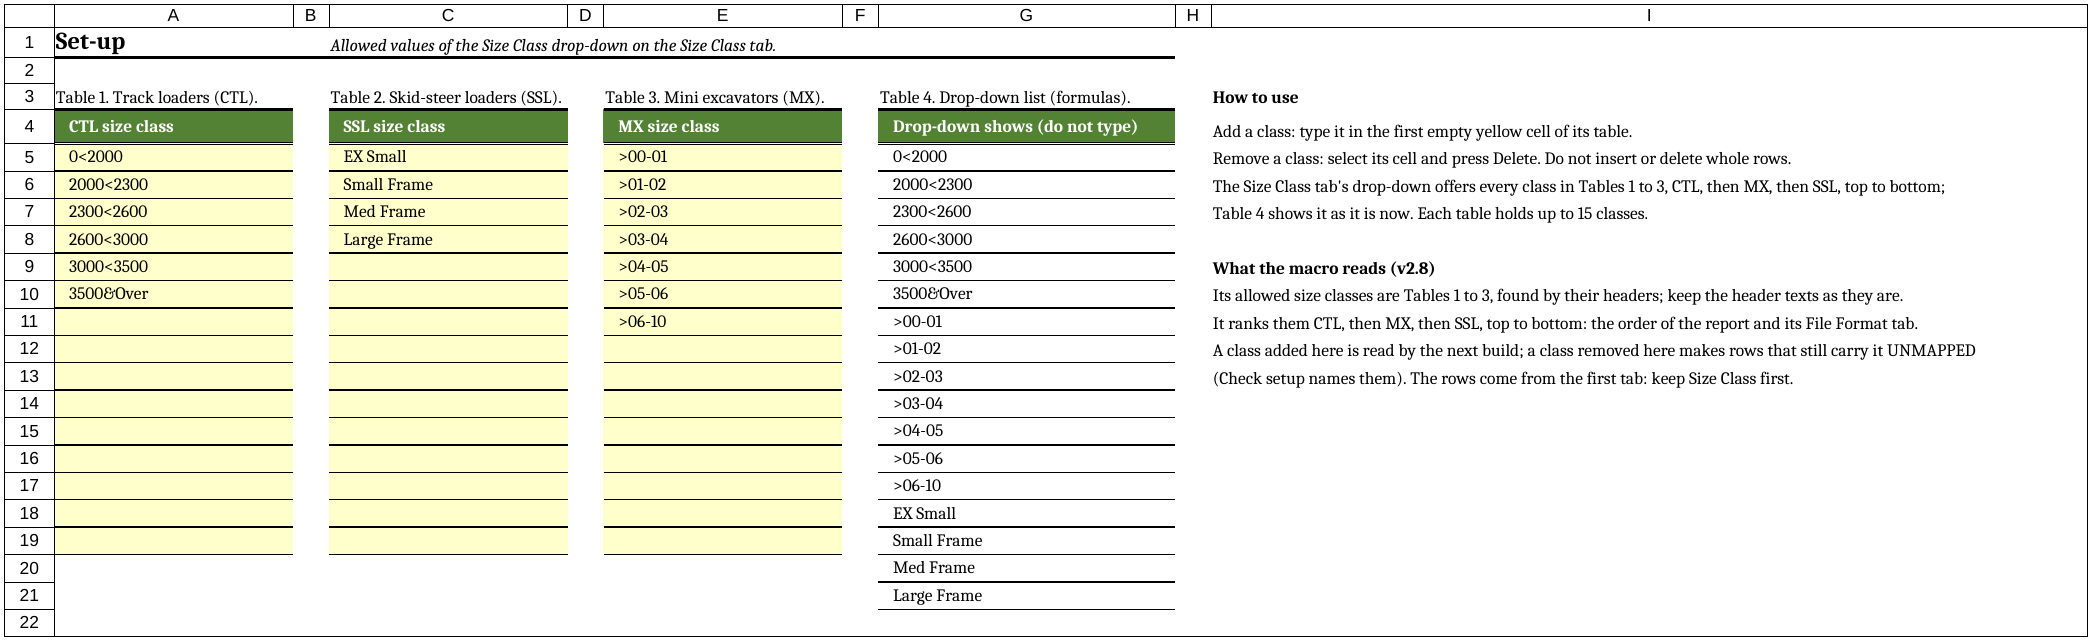
\includegraphics[width=2.55in]{setup-tab.png}\\[4pt]
  \begin{itemize}
  \item Three tables: CTL, SSL, MX
  \item You type the classes in the \yellow{yellow} cells
  \item Builds the list for the drop-down
  \end{itemize}};

\node[station, anchor=north west, text width=2.55in] (h2) at (3.2,6.4) {2\quad Size Class tab};
\node[box, anchor=north, text width=2.55in] (b2) at (h2.south) {\by{Which class each model is in}
  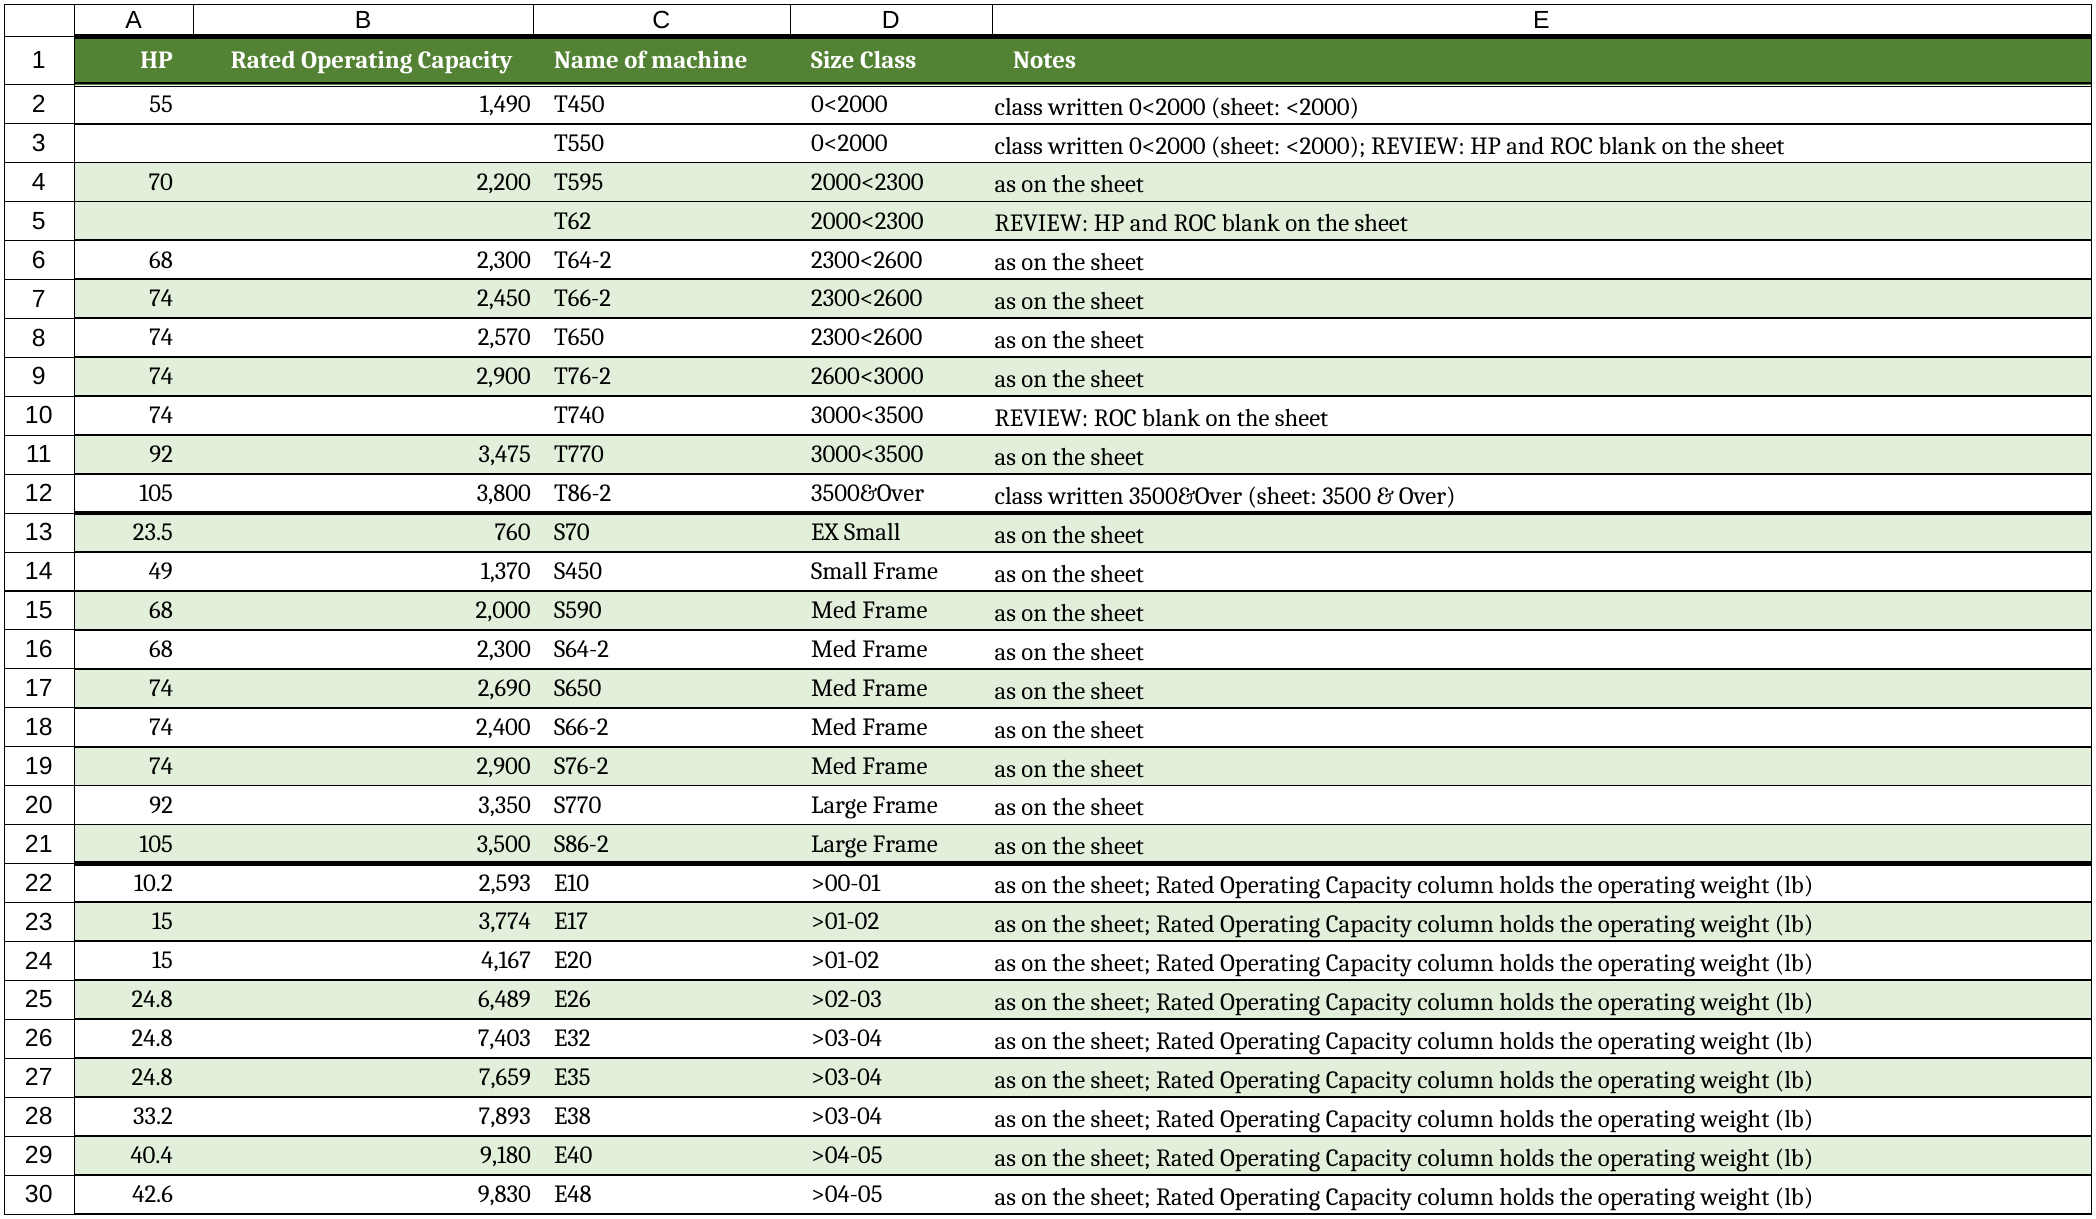
\includegraphics[width=2.55in]{size-class-tab.png}\\[4pt]
  \begin{itemize}
  \item One row per model (29 today)
  \item Name of machine and its Size Class
  \item Size Class is a drop-down of the Set-up classes
  \end{itemize}};

\node[station, anchor=north west, text width=2.4in] (h3) at (6.15,6.4) {3\quad The macro reads it};
\node[box, anchor=north, text width=2.4in] (b3) at (h3.south) {\by{Config sheet of the report builder}
  \begin{itemize}
  \item \btn{Choose size class file...} points the macro at this workbook (setting \texttt{SizeClassFile})
  \item \btn{Check setup} reads both tabs and lists anything wrong, without building
  \item \btn{Build report} reads them again, then builds
  \end{itemize}};

\node[station, anchor=north west, text width=2.55in] (h4) at (8.95,6.4) {4\quad The report uses it};
\node[box, anchor=north, text width=2.55in] (b4) at (h4.south) {\by{Every order row gets a class}
  \begin{itemize}
  \item Each order's MODEL\_GROUP is looked up by Name of machine
  \item Rows sorted by class: CTL, then MX, then SSL, in the Set-up order
  \item A model not on the list is \peach{UNMAPPED} and sorted last
  \end{itemize}};

\draw[flow] (h1.east) -- (h2.west);
\draw[flow] (h2.east) -- (h3.west);
\draw[flow] (h3.east) -- (h4.west);

% ---------------------------------------------------------------- the three families
\node[anchor=north west, inner sep=0pt, font=\sffamily\bfseries\small] at (6.15,3.7) {The three families};
\draw[line width=0.8pt] (6.15,3.45) -- (11.5,3.45);
\node[anchor=north west, inner sep=0pt, font=\sffamily\footnotesize] at (6.15,3.38) {%
  \renewcommand{\arraystretch}{1.35}%
  \begin{tabular}{@{}p{0.55in}p{1.45in}p{1.6in}p{1.4in}@{}}
  \textbf{Family} & \textbf{Machines} & \textbf{Class by} & \textbf{Example class} \\ \hline
  CTL & Compact track loaders & Rated operating capacity, lb & \cls{2000<2300} \\
  SSL & Skid-steer loaders & Frame size & \cls{Med Frame} \\
  MX  & Mini excavators & Operating weight, tonnes & \cls{>01-02} \\ \hline
  \end{tabular}};

% ---------------------------------------------------------------- this guide
\node[anchor=north west, inner sep=0pt, font=\sffamily\bfseries\small] at (0.25,2.55) {In this guide};
\draw[line width=0.8pt] (0.25,2.3) -- (5.45,2.3);
\node[anchor=north west, inner sep=0pt, align=left, font=\sffamily\footnotesize] at (0.25,2.2) {%
  \renewcommand{\arraystretch}{1.3}%
  \begin{tabular}{@{}p{0.55in}l@{}}
  Sheet 1 & The file at a glance (this sheet) \\
  Sheet 2 & The Size Class tab: one row per model \\
  Sheet 3 & The Set-up tab: the list of classes \\
  Sheet 4 & How the macro reads the file, and what its messages mean \\
  \textbf{Sheet 5} & \textbf{Add a new size class to CTL, SSL or MX} \\
  \end{tabular}};

% ---------------------------------------------------------------- the most important job
\node[anchor=north west, draw=alertorange, line width=2pt, fill=flagpeach, text width=5.15in, align=left,
      inner sep=8pt] at (6.15,2.05)
  {{\bfseries\large Most important job: add a new size class}\hfill{\bfseries Sheet 5}\\[5pt]
   Set-up tab: type the class in the first empty yellow cell of its table (CTL, SSL or MX).
   It appears in the drop-down at once; pick it for its models on the Size Class tab, save,
   then \btn{Check setup} on Config.};

\titleblock{At a Glance}{1 of 5}
\end{tikzpicture}}

\newpage
% ============================================================================ sheet 2: the Size Class tab
% picture: 2096 x 1219 px, 7.0 in wide, so 4.071 in high, top left at (0.75,6.4)
\noindent
\scalebox{1.333333}{%
\begin{tikzpicture}[x=1in, y=1in]
\useasboundingbox (0,0) rectangle (12,7.5);
\draw[line width=0.8pt] (0,0) rectangle (12,7.5);
\heading{Size Class Tab}
  {The first tab: one row per model. The macro reads two columns, Name of machine and Size Class.}

\node[shot] (img) at (0.75,6.4) {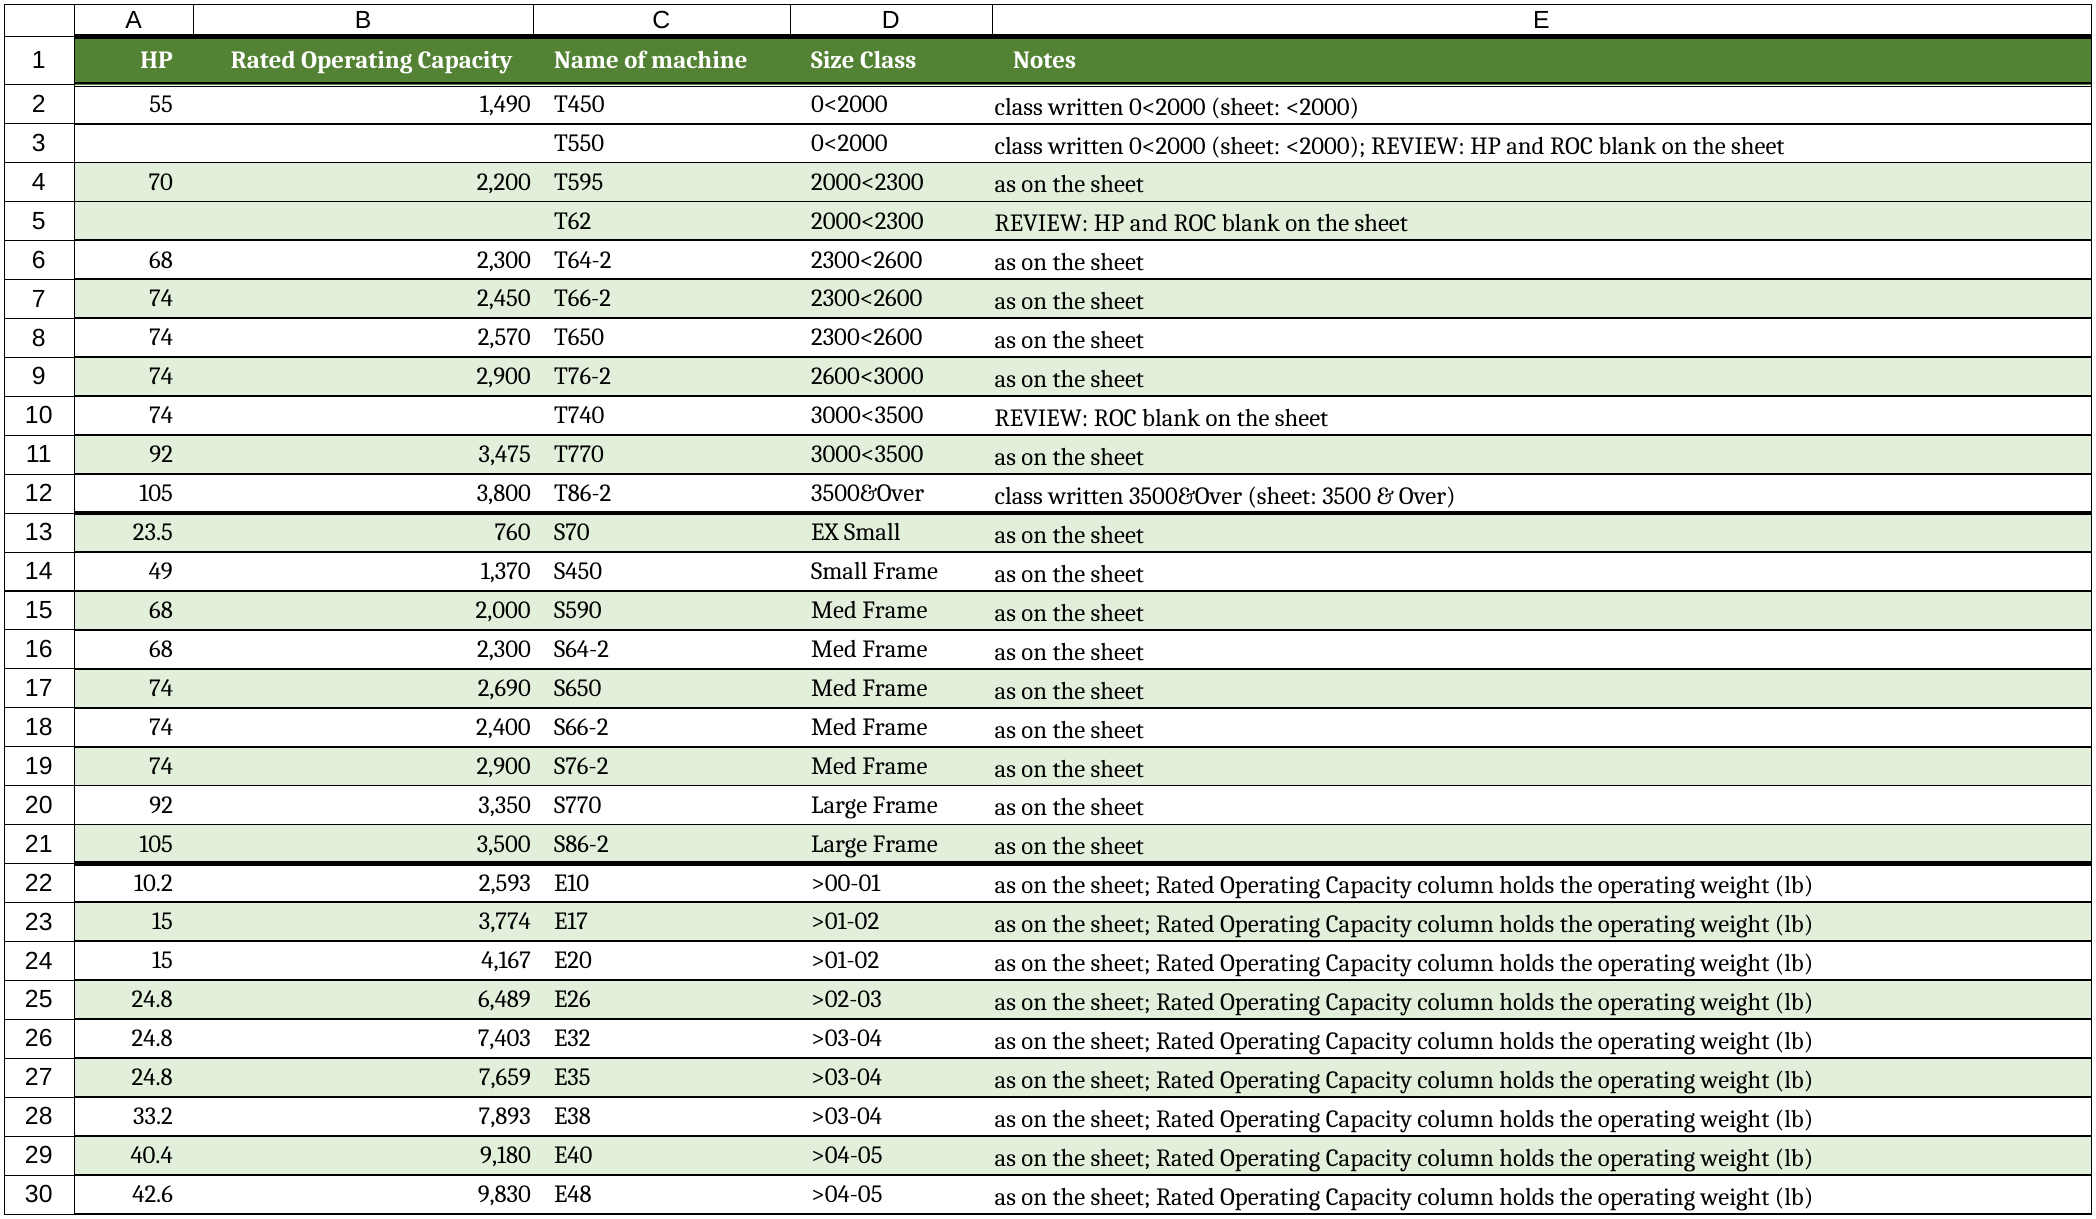
\includegraphics[width=7.0in]{size-class-tab.png}};
\begin{scope}[shift={(0.75,6.4)}, x=7.0in, y=-4.071in]
  % markers above the column letters
  \foreach \fx/\n in {0.063/1, 0.173/2, 0.316/3, 0.426/4, 0.737/5} \node[marker] at (\fx,-0.045) {\n};
  % the three family blocks, bracketed on the left
  \foreach \ya/\yb/\t in {0.071/0.418/CTL, 0.424/0.706/SSL, 0.712/0.997/MX} {
    \draw[line width=0.8pt] (-0.012,\ya) -- (-0.03,\ya) -- (-0.03,\yb) -- (-0.012,\yb);
    \node[rotate=90, font=\sffamily\bfseries\small, inner sep=0pt] at (-0.052,{(\ya+\yb)/2}) {\t};
  }
\end{scope}

% ---------------------------------------------------------------- the five columns
\node[anchor=north west, align=left, text width=3.6in, inner sep=0pt] at (8.05,6.4) {%
  \textbf{\large The five columns}\\[6pt]
  \num{1}\enspace\textbf{HP}\\[1pt]
  {\footnotesize For people. The macro does not read it.}\\[6pt]
  \num{2}\enspace\textbf{Rated Operating Capacity}\\[1pt]
  {\footnotesize Loaders: rated operating capacity in lb. Excavators: operating weight in lb.
   Use it to decide the class; the macro does not read it.}\\[6pt]
  \num{3}\enspace\textbf{Name of machine}\quad{\footnotesize\itshape read by the macro}\\[1pt]
  {\footnotesize Must match the MODEL\_GROUP in the Order Intake export, e.g.\ \cls{T770}. Case does not matter.
   Extra words after the name are fine: \cls{T740 Compact Track Loader} matches \cls{T740}.}\\[6pt]
  \num{4}\enspace\textbf{Size Class}\quad{\footnotesize\itshape read by the macro}\\[1pt]
  {\footnotesize Pick it from the drop-down. Excel refuses any class that is not on the Set-up tab (Sheet 3).}\\[6pt]
  \num{5}\enspace\textbf{Notes}\\[1pt]
  {\footnotesize For people. \cls{REVIEW:} marks a row with a figure still to confirm (T550, T62, T740).}};

% ---------------------------------------------------------------- add a model; good to know
\node[station, anchor=north west, text width=3.4in] (ha) at (0.25,2.1) {Add a new model};
\node[box, anchor=north, text width=3.4in] at (ha.south) {%
  \begin{enumerate}[leftmargin=1.2em, labelsep=0.4em, itemsep=2pt, topsep=0pt, parsep=0pt]
  \item Go to the first empty row under the table (row 31 today).
  \item Type the model in \textbf{Name of machine}, as the export spells it.
  \item Pick its class in \textbf{Size Class}. Not in the list? Add the class first (Sheet 5).
  \item HP, capacity and Notes are optional. Save.
  \end{enumerate}};

\node[station, anchor=north west, text width=3.9in] (hg) at (4.05,2.1) {Good to know};
\node[box, anchor=north, text width=3.9in] at (hg.south) {%
  \begin{itemize}
  \item Row order does not matter; the report sorts by class. The rows are grouped by family only to read easily.
  \item A model listed twice: the first row is used, the other is reported.
  \item Keep the header texts in row 1, and keep this tab first in the workbook.
  \end{itemize}};

\titleblock{Size Class Tab}{2 of 5}
\end{tikzpicture}}

\newpage
% ============================================================================ sheet 3: the Set-up tab
% picture: 2092 x 641 px, 11.5 in wide, so 3.524 in high, top left at (0.25,6.45)
\noindent
\scalebox{1.333333}{%
\begin{tikzpicture}[x=1in, y=1in]
\useasboundingbox (0,0) rectangle (12,7.5);
\draw[line width=0.8pt] (0,0) rectangle (12,7.5);
\heading{Set-up Tab}
  {The second tab: the size classes that exist. Tables 1 to 3 are typed by you; Table 4 builds itself and feeds the drop-down.}

\node[shot] at (0.25,6.45) {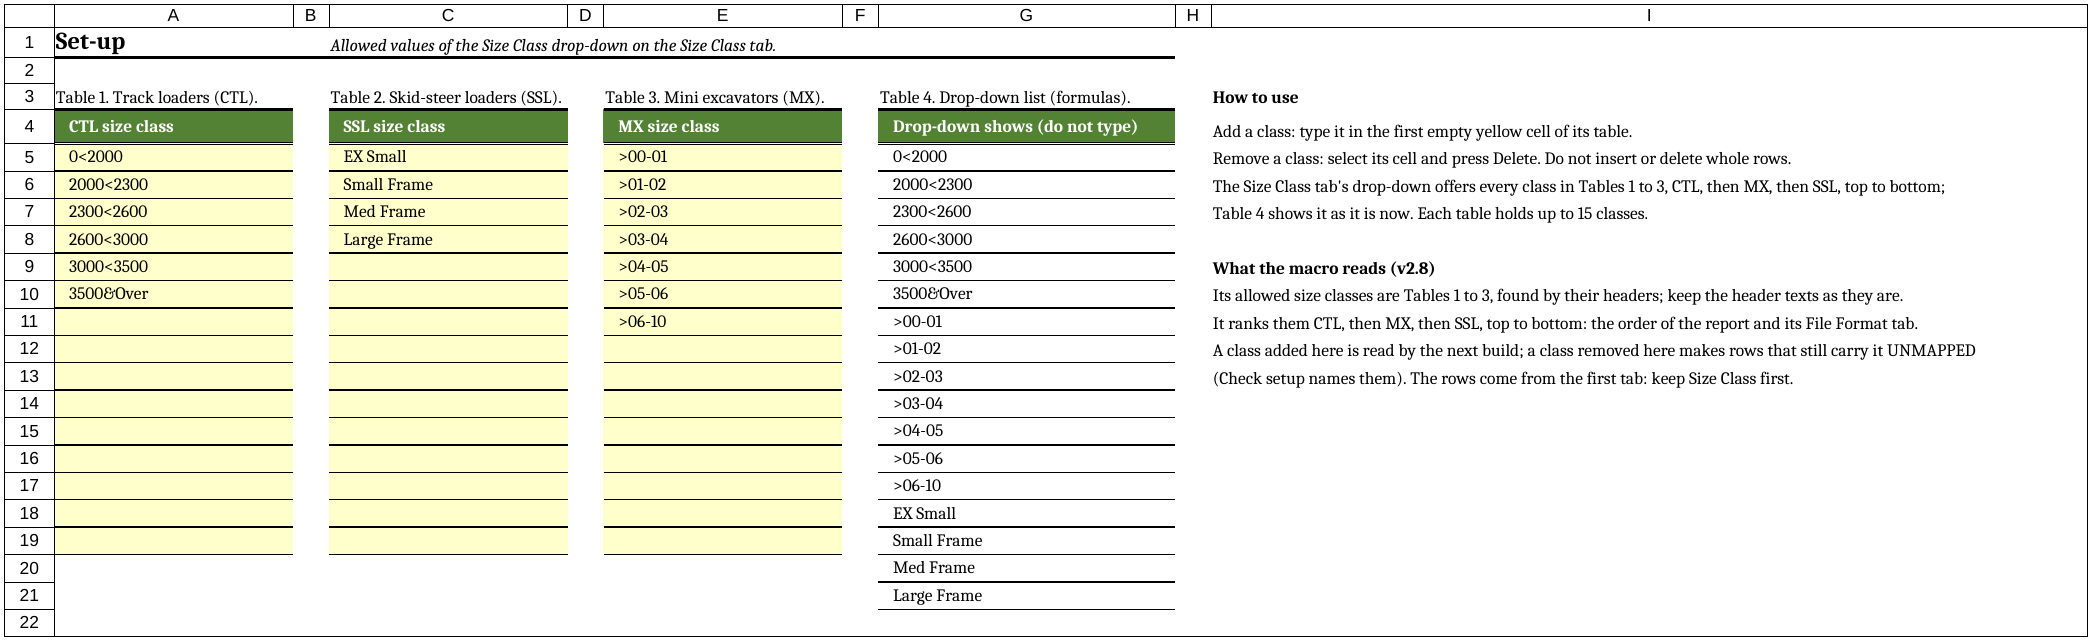
\includegraphics[width=11.5in]{setup-tab.png}};
\begin{scope}[shift={(0.25,6.45)}, x=11.5in, y=-3.524in]
  \node[marker] at (0.12,0.19) {A};
  \node[marker] at (0.255,0.19) {A};
  \node[marker] at (0.385,0.19) {A};
  \node[marker] at (0.567,0.19) {B};
  \node[marker] at (0.03,0.55) {C};
  \draw[flow, headgreen] (0.03,0.6) -- (0.03,0.85);
\end{scope}

% ---------------------------------------------------------------- what each part is
\node[station, anchor=north west, text width=2.55in] (ha) at (0.25,2.75) {\num{A}\enspace Tables 1 to 3: you type};
\node[box, anchor=north, text width=2.55in] at (ha.south) {%
  \begin{itemize}
  \item One table per family: CTL (column A), SSL (C), MX (E)
  \item One class per \yellow{yellow} cell, spelled as the report should show it
  \item 15 cells per table
  \item Keep the green header texts exactly: the macro finds the tables by them
  \end{itemize}};

\node[station, anchor=north west, text width=2.55in] (hb) at (3.2,2.75) {\num{B}\enspace Table 4: do not type};
\node[box, anchor=north, text width=2.55in] at (hb.south) {%
  \begin{itemize}
  \item Formulas stack Tables 1 to 3 into one list: CTL, then MX, then SSL; blanks skipped
  \item This list is the Size Class drop-down
  \item It updates as you type in Tables 1 to 3
  \end{itemize}};

\node[station, anchor=north west, text width=2.55in] (hc) at (6.15,2.75) {\num{C}\enspace Order matters};
\node[box, anchor=north, text width=2.55in] at (hc.south) {%
  \begin{itemize}
  \item Top to bottom in a table is the order in the report and on its File Format tab
  \item Keep each table smallest to largest
  \item The tab shows SSL in the middle; the report still puts MX before SSL
  \end{itemize}};

\node[station, anchor=north west, text width=2.55in] (hd) at (9.1,2.75) {Remove or rename a class};
\node[box, anchor=north, text width=2.55in] at (hd.south) {%
  \begin{itemize}
  \item Remove: select the cell, press Delete. Never insert or delete whole rows
  \item Models still showing the old class are skipped and end up \peach{UNMAPPED}: pick a new class for them
  \item Rename: add the new name, re-pick it for the models, delete the old one
  \end{itemize}};

\titleblock{Set-up Tab}{3 of 5}
\end{tikzpicture}}

\newpage
% ============================================================================ sheet 4: how the macro reads it
\noindent
\scalebox{1.333333}{%
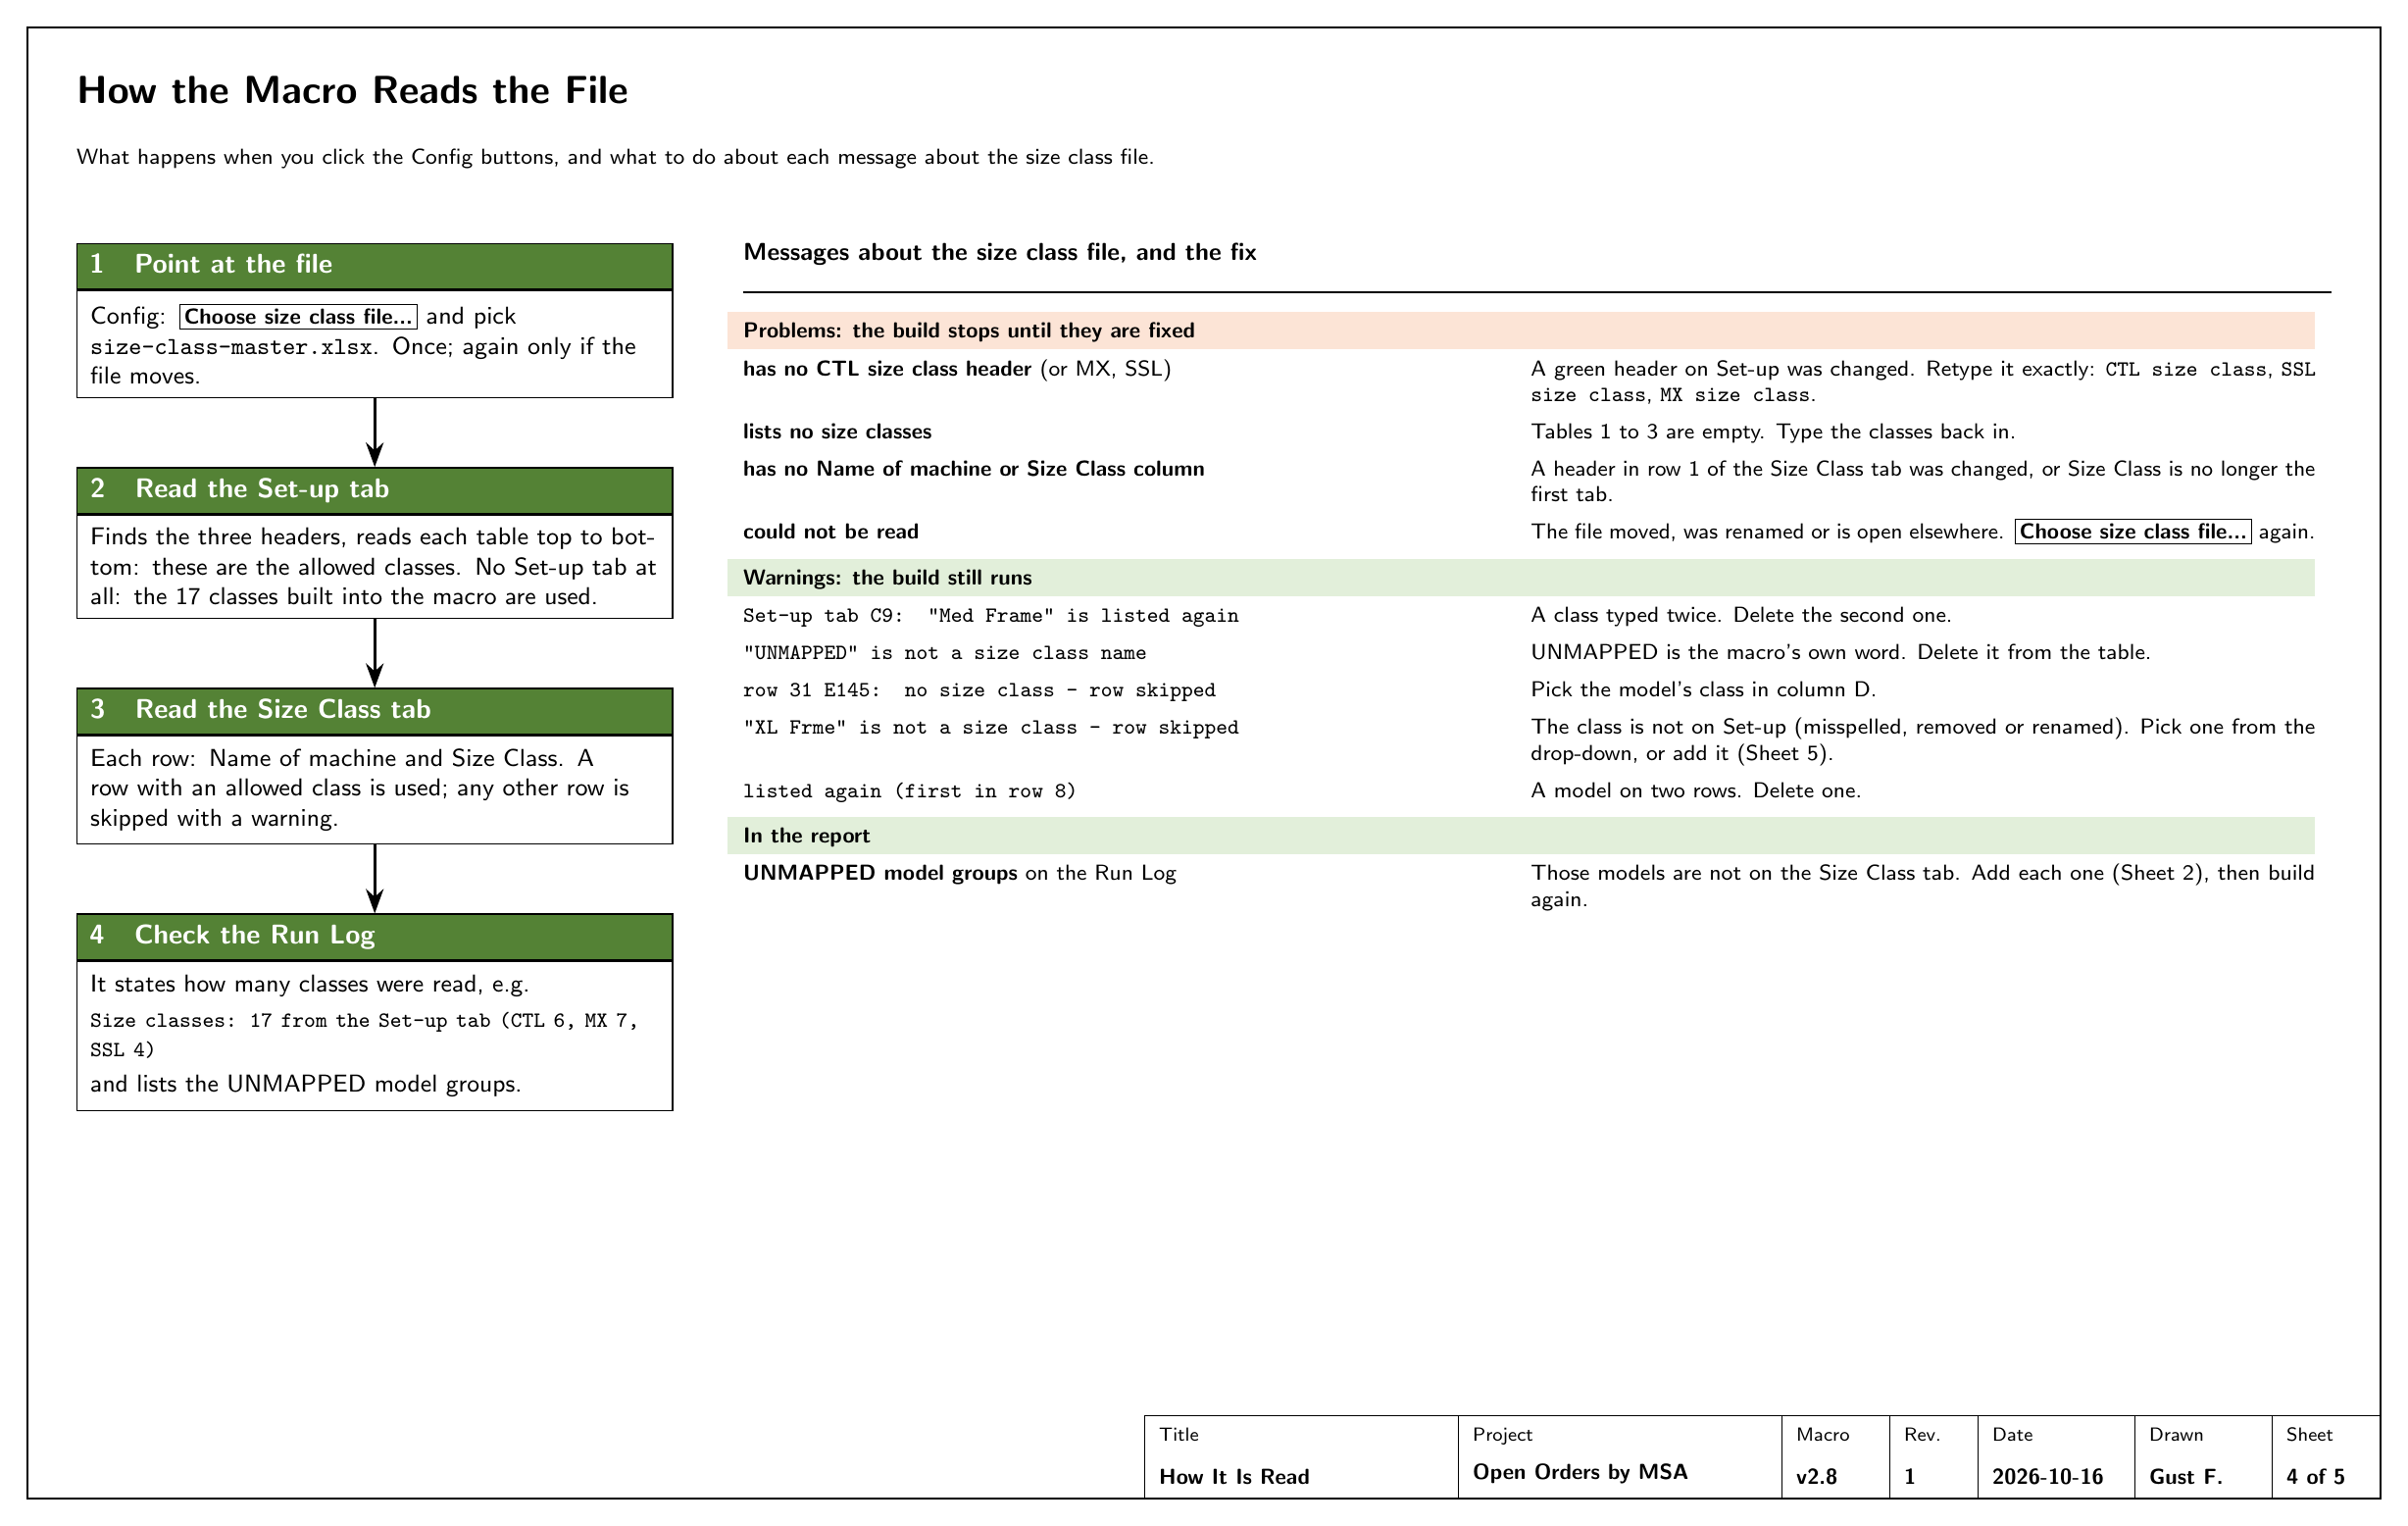
\begin{tikzpicture}[x=1in, y=1in]
\useasboundingbox (0,0) rectangle (12,7.5);
\draw[line width=0.8pt] (0,0) rectangle (12,7.5);
\heading{How the Macro Reads the File}
  {What happens when you click the Config buttons, and what to do about each message about the size class file.}

% ---------------------------------------------------------------- the read, top to bottom
\node[station, anchor=north west, text width=2.9in] (s1) at (0.25,6.4) {1\quad Point at the file};
\node[box, anchor=north, text width=2.9in] (t1) at (s1.south) {%
  Config: \btn{Choose size class file...} and pick \texttt{size-class-master.xlsx}. Once; again only if the file moves.};
\node[station, anchor=north west, text width=2.9in] (s2) at ($(t1.south west)+(0,-0.35)$) {2\quad Read the Set-up tab};
\node[box, anchor=north, text width=2.9in] (t2) at (s2.south) {%
  Finds the three headers, reads each table top to bottom: these are the allowed classes.
  No Set-up tab at all: the 17 classes built into the macro are used.};
\node[station, anchor=north west, text width=2.9in] (s3) at ($(t2.south west)+(0,-0.35)$) {3\quad Read the Size Class tab};
\node[box, anchor=north, text width=2.9in] (t3) at (s3.south) {%
  Each row: Name of machine and Size Class. A row with an allowed class is used; any other row is skipped with a warning.};
\node[station, anchor=north west, text width=2.9in] (s4) at ($(t3.south west)+(0,-0.35)$) {4\quad Check the Run Log};
\node[box, anchor=north, text width=2.9in] (t4) at (s4.south) {%
  It states how many classes were read, e.g.\\[2pt]
  {\footnotesize\ttfamily Size classes: 17 from the Set-up tab (CTL 6, MX 7, SSL 4)}\\[2pt]
  and lists the UNMAPPED model groups.};
\draw[flow] (t1.south) -- (s2.north);
\draw[flow] (t2.south) -- (s3.north);
\draw[flow] (t3.south) -- (s4.north);

% ---------------------------------------------------------------- the messages
\node[anchor=north west, inner sep=0pt, font=\sffamily\bfseries\small] at (3.65,6.4) {Messages about the size class file, and the fix};
\draw[line width=0.8pt] (3.65,6.15) -- (11.75,6.15);
\node[anchor=north west, inner sep=0pt, font=\sffamily\footnotesize] at (3.65,6.05) {%
  \renewcommand{\arraystretch}{1.45}%
  \begin{tabular}{@{}p{3.85in}p{4.0in}@{}}
  \multicolumn{2}{@{}l}{\cellcolor{flagpeach}\textbf{Problems: the build stops until they are fixed}}\\
  \textbf{has no CTL size class header} (or MX, SSL) & A green header on Set-up was changed. Retype it exactly: \cls{CTL size class}, \cls{SSL size class}, \cls{MX size class}. \\
  \textbf{lists no size classes} & Tables 1 to 3 are empty. Type the classes back in. \\
  \textbf{has no Name of machine or Size Class column} & A header in row 1 of the Size Class tab was changed, or Size Class is no longer the first tab. \\
  \textbf{could not be read} & The file moved, was renamed or is open elsewhere. \btn{Choose size class file...} again. \\[3pt]
  \multicolumn{2}{@{}l}{\cellcolor{bandgreen}\textbf{Warnings: the build still runs}}\\
  {\ttfamily Set-up tab C9: "Med Frame" is listed again} & A class typed twice. Delete the second one. \\
  {\ttfamily "UNMAPPED" is not a size class name} & UNMAPPED is the macro's own word. Delete it from the table. \\
  {\ttfamily row 31 E145: no size class - row skipped} & Pick the model's class in column D. \\
  {\ttfamily "XL Frme" is not a size class - row skipped} & The class is not on Set-up (misspelled, removed or renamed). Pick one from the drop-down, or add it (Sheet 5). \\
  {\ttfamily listed again (first in row 8)} & A model on two rows. Delete one. \\[3pt]
  \multicolumn{2}{@{}l}{\cellcolor{bandgreen}\textbf{In the report}}\\
  \textbf{UNMAPPED model groups} on the Run Log & Those models are not on the Size Class tab. Add each one (Sheet 2), then build again. \\
  \end{tabular}};

\titleblock{How It Is Read}{4 of 5}
\end{tikzpicture}}

\newpage
% ============================================================================ sheet 5: add a new size class
% pictures: setup-after 2062 x 1116 px, 6.6 in wide, so 3.572 in high, top left at (5.15,6.0);
%           size-class-new 1907 x 395 px, 6.6 in wide, so 1.367 in high, top left at (5.15,1.95)
\noindent
\scalebox{1.333333}{%
\begin{tikzpicture}[x=1in, y=1in]
\useasboundingbox (0,0) rectangle (12,7.5);
\draw[line width=3pt, alertorange] (0,0) rectangle (12,7.5);
\node[anchor=north west, inner sep=0pt, font=\sffamily\bfseries\fontsize{14}{16}\selectfont]
  at (0.25,7.25) {Add a New Size Class: CTL, SSL, MX};
\node[anchor=north east, fill=alertorange, text=white, font=\sffamily\bfseries\normalsize, inner sep=5pt]
  at (11.75,7.28) {THE MOST IMPORTANT JOB};
\node[anchor=north west, inner sep=0pt, font=\sffamily\footnotesize] at (0.25,6.88)
  {The same steps for all three families; only the table changes. Example: \cls{4000\&Over} (CTL), \cls{XL Frame} (SSL),
   \cls{>10-15} (MX), shaded \peach{peach} in the pictures. Use the class names your size class slide gives.};

% ---------------------------------------------------------------- the steps
\node[station, anchor=north west, text width=4.45in] (s1) at (0.25,6.45) {\hotnum{1}\enspace Open the file, go to the Set-up tab};

\node[station, anchor=north west, text width=4.45in] (s2) at ($(s1.south west)+(0,-0.12)$) {\hotnum{2}\enspace Find the table of the family};
\node[box, anchor=north, text width=4.45in, font=\sffamily\footnotesize] (t2) at (s2.south) {%
  \renewcommand{\arraystretch}{1.2}%
  \begin{tabular}{@{}p{0.5in}p{1.5in}p{0.7in}p{1.3in}@{}}
  \textbf{CTL} & Table 1 & column \textbf{A} & e.g.\ \cls{4000\&Over} \\
  \textbf{SSL} & Table 2 & column \textbf{C} & e.g.\ \cls{XL Frame} \\
  \textbf{MX}  & Table 3 & column \textbf{E} & e.g.\ \cls{>10-15} \\
  \end{tabular}};

\node[station, anchor=north west, text width=4.45in] (s3) at ($(t2.south west)+(0,-0.12)$) {\hotnum{3}\enspace Type the class in the first empty yellow cell};
\node[box, anchor=north, text width=4.45in] (t3) at (s3.south) {%
  \begin{itemize}
  \item Spell it as the report should show it; one class per cell
  \item Largest class? It goes at the bottom, as in the example
  \item Belongs between two classes? Select the cells from that spot down to the last class, drag their
        border one cell down, then type in the gap. Never insert whole rows
  \end{itemize}};

\node[station, anchor=north west, text width=4.45in] (s4) at ($(t3.south west)+(0,-0.12)$) {\hotnum{4}\enspace Check Table 4 (column G)};
\node[box, anchor=north, text width=4.45in] (t4) at (s4.south) {%
  The new class shows in its place in the list: it is now in the drop-down.};

\node[station, anchor=north west, text width=4.45in] (s5) at ($(t4.south west)+(0,-0.12)$) {\hotnum{5}\enspace Give it to the models, on the Size Class tab};
\node[box, anchor=north, text width=4.45in] (t5) at (s5.south) {%
  Pick the new class in column D for each model in it; a new model goes in the first empty row (Sheet 2). Save and close.};

\node[station, anchor=north west, text width=4.45in] (s6) at ($(t5.south west)+(0,-0.12)$) {\hotnum{6}\enspace Config: \btn{Check setup}, then \btn{Build report}};
\node[box, anchor=north, text width=4.45in] (t6) at (s6.south) {%
  The Run Log counts the new classes (the example):
  {\footnotesize\ttfamily Size classes: 20 from the Set-up tab (CTL 7, MX 8, SSL 5)}};

% ---------------------------------------------------------------- the Set-up tab after step 3
\node[anchor=south west, inner sep=0pt, font=\sffamily\bfseries\small] at (5.15,6.08) {Set-up tab after step 3};
\node[shot] at (5.15,6.0) {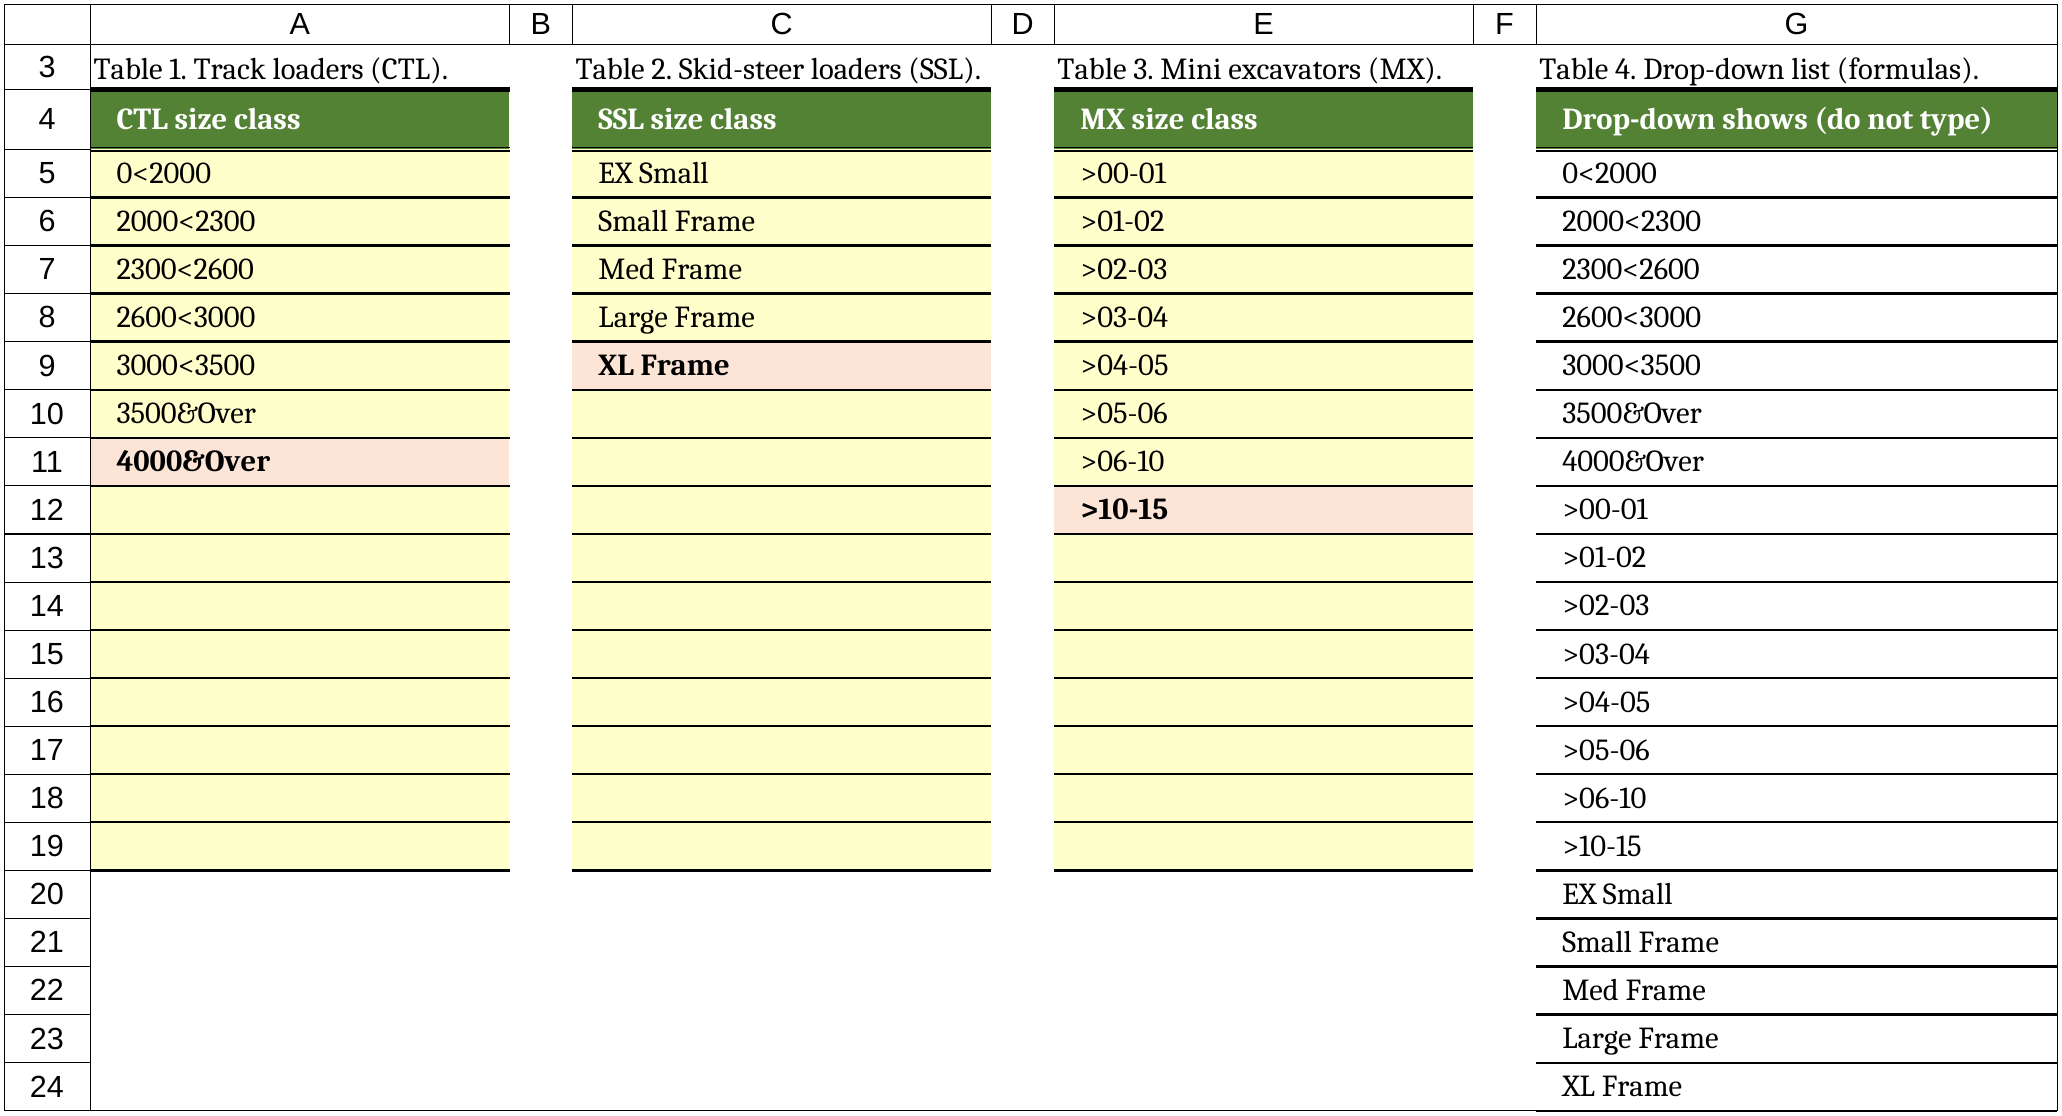
\includegraphics[width=6.6in]{setup-after.png}};
\begin{scope}[shift={(5.15,6.0)}, x=6.6in, y=-3.572in]
  % step 3: the three cells typed (A11, C9, E12)
  \node[hot] at (0.215,0.412) {3};
  \node[hot] at (0.448,0.327) {3};
  \node[hot] at (0.681,0.456) {3};
  % step 4: where they show in Table 4 (G11, G19, G24)
  \foreach \fy in {0.412, 0.757, 0.972} \draw[line width=1.4pt, alertorange] (0.745,\fy-0.021) rectangle (0.995,\fy+0.021);
  \node[hot] at (0.70,0.757) {4};
  \foreach \fy in {0.412, 0.757, 0.972} \draw[point] (0.70,0.757) ++(0.012,{0.02*sign(\fy-0.757)}) -- (0.743,\fy);
\end{scope}

% ---------------------------------------------------------------- the Size Class tab after step 5
\node[anchor=south west, inner sep=0pt, font=\sffamily\bfseries\small] at (5.15,2.03) {Size Class tab after step 5 (header and last rows)};
\node[shot] at (5.15,1.95) {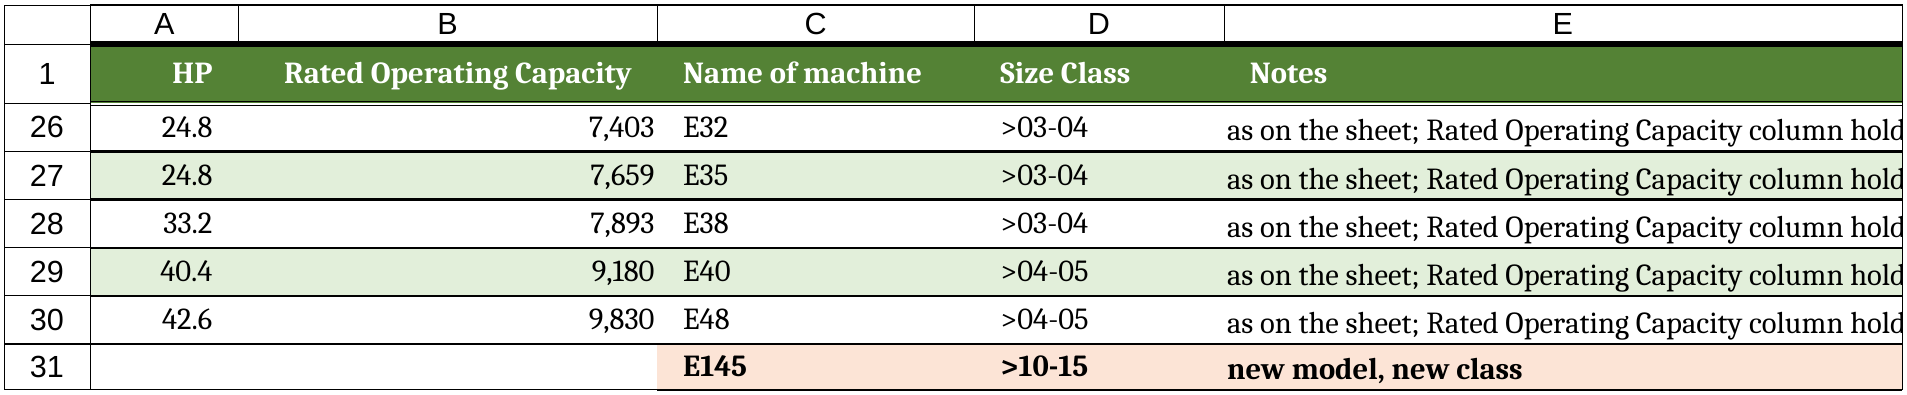
\includegraphics[width=6.6in]{size-class-new.png}};
\begin{scope}[shift={(5.15,1.95)}, x=6.6in, y=-1.367in]
  \node[hot] at (0.495,0.927) {5};
\end{scope}

% ---------------------------------------------------------------- the don'ts
\node[anchor=north west, draw, line width=0.5pt, fill=flagpeach, text width=4.45in, align=left, font=\sffamily\footnotesize]
  at ($(t6.south west)+(0,-0.2)$) {\textbf{Do not:} type in Table 4, change the green headers, insert or delete whole rows,
  or type a class twice or the word UNMAPPED. Up to 15 classes per table.};

\titleblock{Add a Size Class}{5 of 5}
\end{tikzpicture}}
\end{document}
